\documentclass[10pt,a4paper,notitlepage]{report}
\usepackage[utf8]{inputenc}
\usepackage{amsmath}
\usepackage{amsfonts}
\usepackage{amssymb}
\usepackage{hyperref}
\usepackage[margin=1in]{geometry}
\usepackage{fancyhdr}
\usepackage[svgnames]{xcolor}
\usepackage{graphicx}

\pagestyle{fancy}
\fancyhead[L]{\small Decoding Neuronal EEG Activity}
\fancyhead[R]{\small\textsc{Problem 3}}
\renewcommand{\headrulewidth}{0.4pt}
\fancyfoot[C]{\thepage}

%\newcommand{\code}[1]{\colorbox{lightgray}{\texttt{#1}}}

\begin{document}

??? GENERAL NOTES ON SUBMISSION, GRADING, ETC. ???

The programming problems consist in filling the gaps in the provided scripts according to the problem description and the comments within the code. The missing parts are typically indicated by '\texttt{...}' (not to be confused with line breaks!), whereas each '\texttt{...}' might be replaced by multiple lines of code. Following the provided code is recommended but only leads you to one of many possible solutions. If some part of the code seems unclear or counterintuitive to you, feel free to depart from it. Be aware, however, that the suggested variable names and structures are typically used later in the script, e. g. for plotting, and occur again in other scripts and problems. In any case, your code should produce the same output as the Musterlösung. \textbf{Note}: To be able to run the code, you must have the folder \texttt{utility} and all subfolders as well as the location of the ECG/EEG datasets added to your MATLAB path.

\section*{Problem}
In this problem, we will analyze and classify human EEG data, analogous to Scheller et al. (2009). Have a look at the paper to get an overview, but be aware that data and processing are not identical to our problem. The data were recorded from one subject under three different levels of anesthesia while constantly presenting short auditory stimuli. Analogous to the ECG data from problem 2, we will eventually try to discriminate data from two arbitrary blocks. However, here we will perform multiresolution analysis (MRA) in order to compute features from the wavelet-transformed signal. The scripts \texttt{runEEG<1,2,3>.m} will successively build the final program, and we will make further adjustments to the classification function, yielding \texttt{modelFitVal3.m}.

\section*{Part 1}
In \texttt{runEEG1.m} we will first examine the data from block 1, corresponding to normal wakefulness. Note that the data are already epoched, yielding the 3 dimensions \textit{channels}, \textit{sample points}, and \textit{epochs}. Each epoch contains 3 consecutive sweeps, i.e. post-stimulus signal sequences, of approx. 102 ms each. Eventually, we will be interested in the middle sweep only.

After specifying the sampling frequency of 5 kHz, loading the signal, and extracting dimensions, the first 3 epochs of all channels of the raw signal will be plotted in a qualitative way. You shouldn't bother understanding exactly what the code does. The plot will give you a general picture of the signal in each channel. After plotting, the code awaits a key press to continue.

The first thing you have to do is build a low-pass filter at approx. 1000 Hz, using \texttt{fdatool} once again. The data are already high-pass filtered, so we only need to apply a low-pass filter. Store the filter object as \texttt{filterLP} under the given file name.

Now we will analyze the data very much like we did in the ECG problem, iterating over all channels. However, be wary of the changed dimensionality of the data. Here, we ''squeeze'' the channel data in order to get rid of the singleton dimension.

First, you have to filter the data. This time, we will only keep one signal. Apply your low-pass filter, then use the function \texttt{cleanAC} (provided in the \texttt{utility} folder) to clean the signal from 50 Hz line noise. Finally, subtract from each epoch its baseline. We define the baseline as the mean signal over a window of 100 points centered at the start of the middle sweep. This should make epochs more comparable. Note that all these computations can be done in matrix form. If you run into trouble, try for-loops instead.

Next, we compute the event-related potential (ERP) for the middle sweep, i.e. we average the middle 512 points of the signal over all epochs. Make sure you average over the correct dimension.

The next line of code computes the wavelet transform and remains unchanged. It calls the function \texttt{MRA\_stationary\_fast} using a Daubechies 4 wavelet to transform the signal at 7 distinct frequency bands, or scales of resolution, centered around approx. 14 Hz, 28 Hz, 56 Hz, 112 Hz, 223 Hz, 446 Hz, and 893 Hz. This is known as multiresolution analysis (MRA). The maximum number of scales is dictated by the length of the signal. (The function actually computes one more scale, but we will only consider the first 7.) This means we get 7 transformed signals for each original signal. These are stored in \texttt{sWT.scales}.

To demonstrate that MRA is a (theoretically) loss-free transformation of the signal, we now reconstruct the signal by adding up the scales one by one. \texttt{WT2ERP} should contain in the $i$th column the sum of scales $1$ to $i$ for the middle sweep, averaged over all epochs.

That's it for part 1. Now your code should produce an overview of all raw channels for the first 3 epochs, followed, after a key press, by a series of figure pairs, advanced at each further key press.

\vspace{1cm}
\hspace{-1cm} 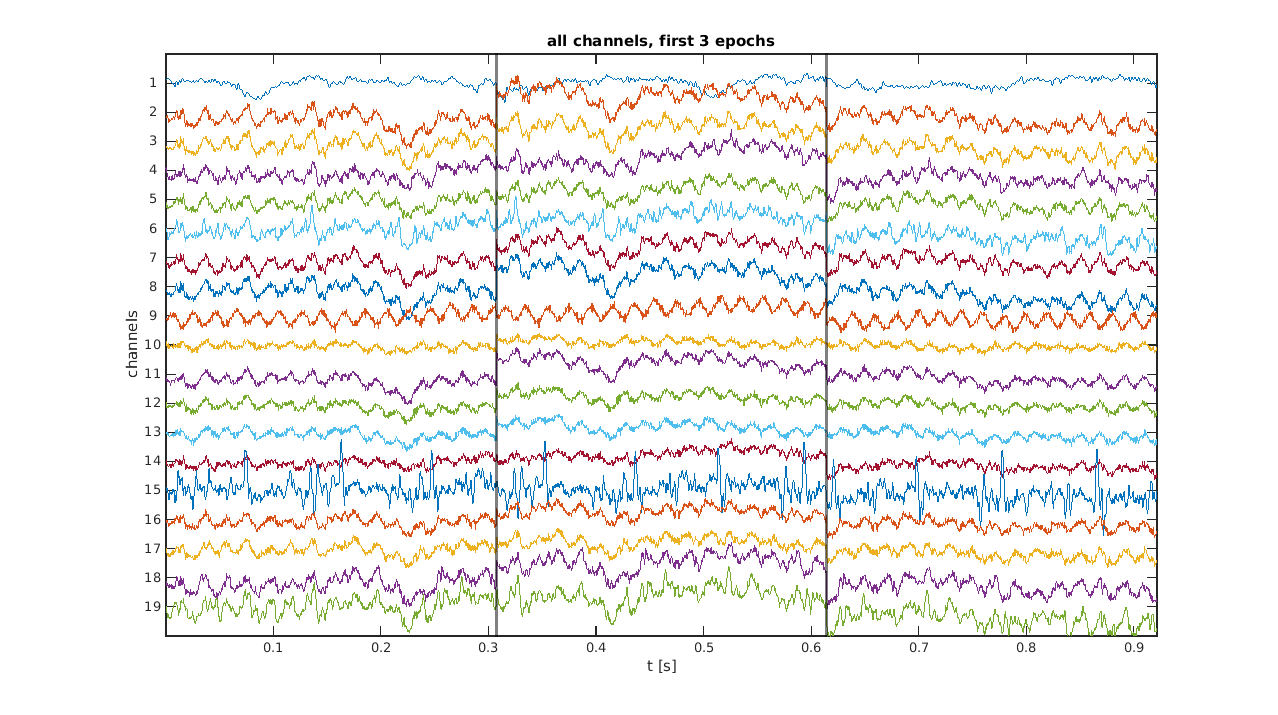
\includegraphics[scale=0.5]{p3fig1.png}

\hspace{-1cm} 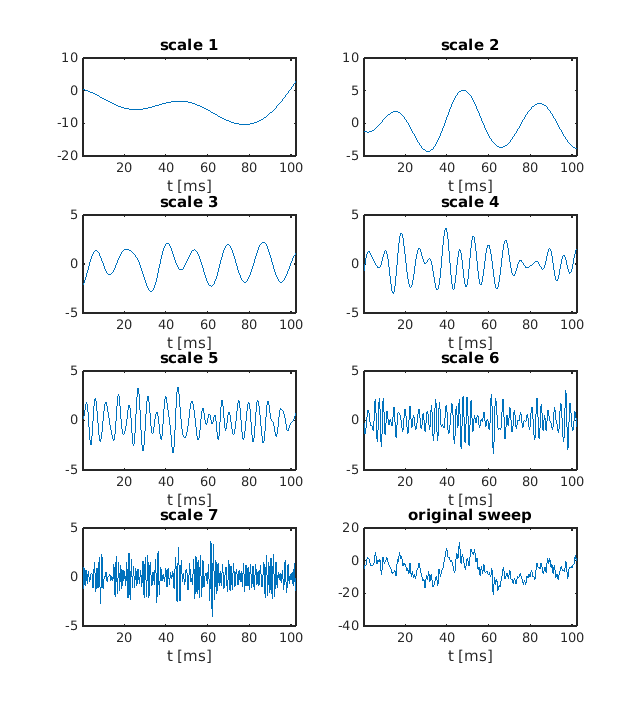
\includegraphics[scale=0.5]{p3fig2.png}
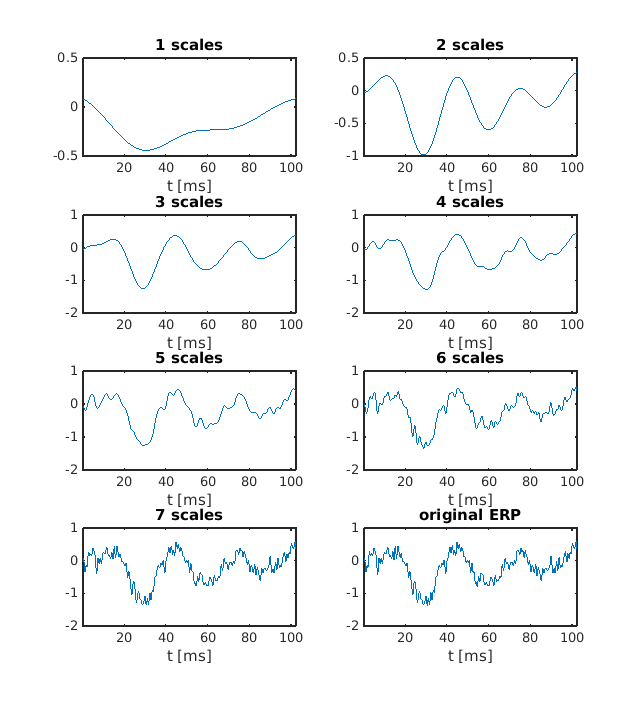
\includegraphics[scale=0.5]{p3fig3.png}
\vspace{5mm}

Each pair of figures shows the wavelet decomposition of the middle sweep of the first epoch of the current channel (left) and the reconstruction of the ERP (right) for the current channel (denoted in the title bars). Note how the reconstruction becomes more and more similar to the original ERP. Also, observe the differences among channels when advancing through the figures. Do some channels look faulty or overly noisy? Re-run the script for blocks 2 and 3.

\section*{Part 2}
In \texttt{runEEG2.m} we will process all 3 blocks and plot some relevant features. We first set a pack size for the computation of PLVs and then specify one channel to use for analysis. Based on your plots from part 1, choose a channel that you think is technically okay in all 3 blocks and representative of the overall signal.

Now we iterate over the 3 blocks, using only the chosen channel. First, filter and baseline-correct the signal as before. The MRA part too is the same as before.

We will now compute instantaneous power and phase. Again, this is very similar to the ECG problem but the data has an additional dimension because we use the 7-fold wavelet transform instead of the signal itself. For each scale separately, power (aka amplitude) is computed as the absolute value of the Hilbert transform, and phase is computed as its angle. Again, unwrap the phase and correct for baseline, i.e. subtract from each epoch its value right before the middle sweep onset. Power will not be baseline-corrected because we're interested in absolute amplitude at the time of the middle sweep.

From the phase you can now compute PLVs. Extend the code from problem 2 by the additional dimension. Again, this is a pointwise operation, so you can process each pack in one go.

The rest is plotting. Your code should produce 3 figures like the one below, each showing, per block, the power, phase, and PLV for the 7 MRA scales. (Only a few of the epochs are plotted for power and phase.)

\vspace{1cm}
\hspace{-1cm} 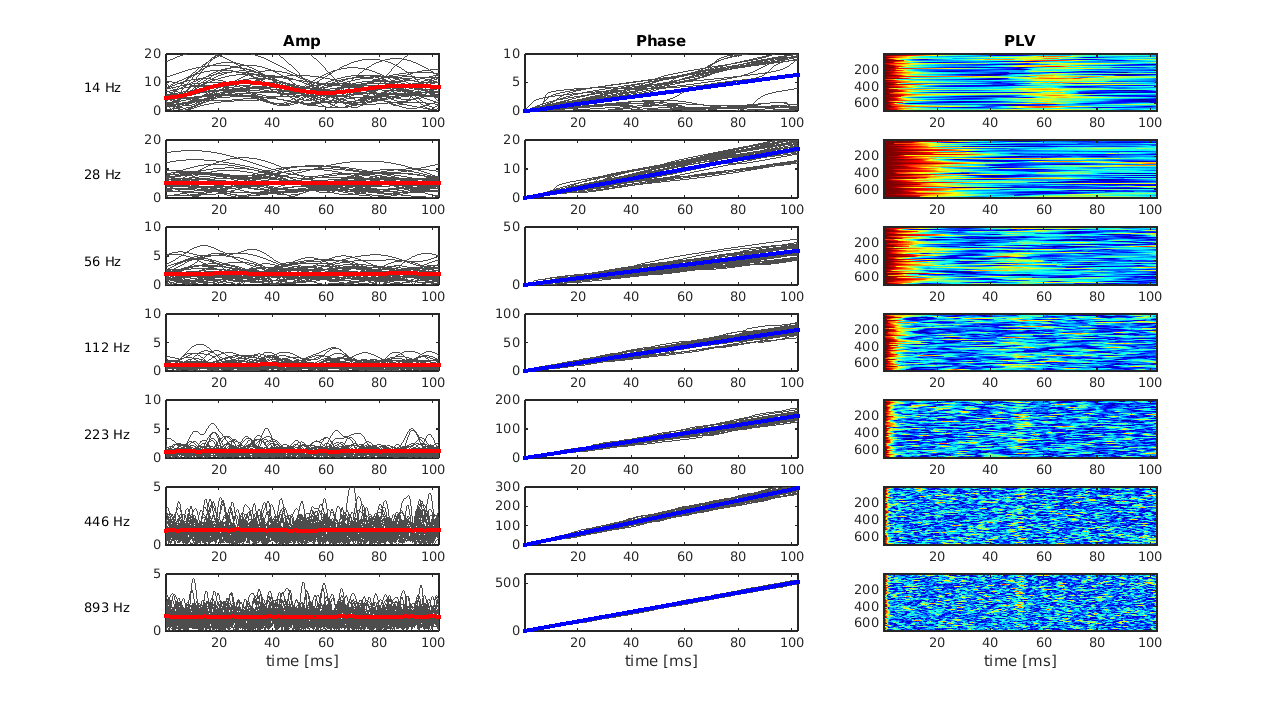
\includegraphics[scale=0.5]{p3fig4.png}
\vspace{5mm}

Compare the 3 blocks, and the scales within each block. Can you make out any differences in frequency content or phase locking strength? You can zoom in on the first 15 ms of all plots by pressing any key.


\section*{Part 3}
In part 3, we will process and classify 2 of the 3 blocks. In \texttt{runEEG3.m}, we specify the 2 blocks and the chosen channel and initialize the features structure (this time we're using only one power feature and one PLV feature).

The analysis section stays the same as in part 2. In the end, we store 2 3D matrices for each block of data.

As with problem 2, we first specify the sweeps (i.e. epochs) to use by limiting the choice to a multiple of \texttt{packSize}. Next, we define some time points from where to sample the features. In consistence with Scheller et al. (2009), let's have a look at wave V of the brainstem auditory evoked potential (BAEP), which appears during the first few milliseconds post-stimulus. You should be able to infer from the paper a set of 5 distinct time points which represent wave V.

Next, specify the set of MRA scales that might be most informative about the level of anesthesia. You might want to start with all 7 scales and sort out the less informative ones, based on your previous plots and some trial and error.

The last thing you have to do in order to successfully run the script is build the feature matrix for the 2 blocks. Each row will contain power and phase locking values for the 5 sample points and the set of scales you chose. The suggested code iterates over scales and simply appends each new set of features to an initially empty matrix. Make sure you rotate, reshape, and repeat the values correctly. Again, if you're unsure, split the problem into further for-loops.

You're basically done. If you run the script you should get the cross-validated performance of the 3 models printed to the command line. Depending on your features, the GLM might yield 100 \% correct classifications. If you're a great deal below that number, try different time points or MRA scales (assuming that your analysis code is correct).

The SVMs on the other hand, especially when using an RBF kernel, could use some tuning. (Again, if they're at 100 \% right away, something is probably wrong.) Have a look into \texttt{modelFitVal3.m}. So far, the function is identical to the Musterlösung from problem 2. Find out how to change the SVM parameters and optimize your classifiers. In the end, your SVMs should classify at least 95 \% of samples correctly.

\end{document}
